\uuid{wFj3}
\exo7id{7282}
\titre{exo7 7282}
\auteur{mourougane}
\organisation{exo7}
\datecreate{2021-08-10}
\isIndication{false}
\isCorrection{false}
\chapitre{Géométrie affine euclidienne}
\sousChapitre{Géométrie affine euclidienne du plan}
\module{Géométrie}
\niveau{L2}
\difficulte{}

\contenu{
\texte{
Étant données trois longueurs \(a\), \(b\) et \(c\), construire à la 
règle et au compas la longueur \(\frac{ab}{c}\). (Indication: on pourra 
considérer la figure ci-dessous.)


\begin{center}
    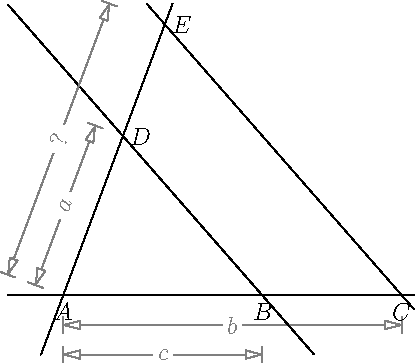
\includegraphics[scale=1]{images/pdf/wFj3-1.pdf}
\end{center}

% [[figure asymptote]]

%\begin{center}
%\begin{asy}
%size(7cm, 0);
%point A = (0, 0); label("\(A\)", A, S);
%point B = (1, 0); label("\(B\)", B, S);
%point C = (1.7, 0); label("\(C\)", C, S);
%line L0 = line(A, B); draw(L0);
%distance("\(b\)", A, C, 5mm, gray);
%distance("\(c\)", A, B, 1cm, gray);
%point D = (0.3, 0.8); label("\(D\)", D, E);
%distance("\(a\)", A, D, -5mm, gray);
%line L1 = line(A, D); draw(L1);
%line L2 = line(B, D); draw(L2);
%line L3 = parallel(C, L2); draw(L3);
%point E0 = intersectionpoint(L1, L3); label("\(E\)", E0, E);
%distance("?", A, E0, -1cm, gray);
%\end{asy}
%\end{center}
}
}
